\documentclass[twocolumn]{aastex63}
\usepackage{natbib}
%\definecolor{orcidlogocol}{HTML}{A6CE39}
\bibliographystyle{aasjournal}

\begin{document}

\title{PLANETESIMAL ACCRETION AT SHORT ORBITAL PERIODS}

\author{Spencer C. Wallace}
\affiliation{Astronomy Department, University of Washington, Seattle, WA 98195}

\author{Thomas R. Quinn}
\affiliation{Astronomy Department, University of Washington, Seattle, WA 98195}

\begin{abstract}
Formation models in which terrestrial bodies grow via the pairwise
accretion of planetesimals have been reasonably successful at
reproducing the general properties of the solar system, including
small body populations. However, planetesimal accretion has not yet
been fully explored in the context of more exotic terrestrial systems,
particularly those that host short-period planets. In this work, we
use direct N-body simulations to explore and understand the growth of
planetary embryos from planetesimals in disks extending down to
$\simeq$ 1 day orbital periods. We show that planetesimal accretion
becomes nearly 100 percent efficient at short orbital periods, leading
to embryo masses that are roughly twice as large as the classical
isolation mass. For rocky bodies, the physical size of the object
begins to occupy a significant fraction of its Hill sphere at orbital
periods less than about 50 days. In this regime, most close encounters
result in collisions, rather than scattering, and the system cannot
bifurcate into a collection of dynamically hot planetesimals and
dynamically cold oligarchs, like is seen in previous work. The highly
efficient accretion seen at short orbital periods implies that systems
of tightly-packed inner planets should be almost completely devoid of
any residual small bodies. We demonstrate the robustness of our
results to assumptions about the initial disk model, and also
investigate how far material can radially mix across the boundary
between modes.
\end{abstract}

%\begin{list}
%\item Explain $\alpha$ controls importance of scattering vs accretion
%\item Also mention $\beta$. Introduces another relevant size scale, but we seem to get runaway growth no matter how large or small this is (is this true?)
%\item Show full disk vhi f6 and f4 simulations. Boundary of efficient accretion moves with density of bodies. Roughly lies where $\alpha = 0.1$.
%\item Eccentricities reach v = vesc regardless of alpha. Show narrow annulus simulations in which embryo 'cools' in planetesimal disk with varying $\alpha$.
%\item Show collision tree plot for full disk vhi f6. Do planetesimals move around much? How does motion of condensation fronts (due to pre-MS evolution of M stars) affect this?
%\item What about fragmentation?
%\item Planetesimals get completely consumed in inner disk. May have implications for planetesimal driven migration (outward, counteract type I migration)?
%\item Embryos form first in the inner disk. What are the implications of this? Might make outward planetesimal driven migration easier
%\end{list}

\section{Introduction} \label{sec:intro}

Planetesimal accretion is a key phase in the terrestrial planet growth
process, bridging the gap from kilometer-sized bodies up to roughly
moon-sized objects known as planetary embryos. In the earliest stages
of the planet formation process, aerodynamic forces dominate the
growth and evolution of the solids and statistical models
\citep{johansen14, birnstiel16} are appropriate to describe how these
numerous, small bodies coagulate. Due to the internal pressure support
of the gas disk, the gas itself orbits at sub-Keplerian speed and
exerts a headwind on any solids large enough to decouple from the gas
\citep{weidenschilling77}. Above about a meter in size, this headwind
is maximally effective at sapping away angular momentum, and planet-building material can fall onto the central star on catastrophically short timescales \citep{weidenschilling77, nakagawa86}. Additionally, laboratory experiments suggest that collisions between mm- to cm- sized solids tend to result in bouncing or destruction, rather than continued growth \citep{blum93, beitz11, colwell03}. For these reasons, a number of mechanisms which involve radially concentrating solids in a planet-forming disk have been proposed to facilitate fast growth from mm to km sizes \citep{johansen07, lyra08, bai10}. Interestingly, formation models for the short-period multiplanet systems revealed by Kepler \citep{fabrycky14} also seem to require enhanced concentrations of planet-building material to reproduce the observed architectures \citep{raymond07, hansen12}.

Regardless of how the mm- to km-sized growth barriers are surmounted, gravity begins to dominate and aerodynamic gas drag plays a less significant role beyond this size. During this phase, collision cross sections are enhanced as gravitational focusing \citep{safronov69} acts to bend the trajectories of bodies undergoing close encounters. Because larger bodies are more effective at focusing the trajectories of nearby planetesimals, a period of runaway growth occurs \citep{wetherill89, kokubo96, barnes09}. Eventually, the largest bodies (known as oligarchs) dynamically heat the surrounding planetesimals, severely limiting further growth \citep{kokubo98}. The end result of this phase is a bimodal population of dynamically cold oligarchs, surrounded by dynamically hot, difficult to accrete residual planetesimals. Lines of evidence suggest that the asteroid belt, Kuiper belt and the Oort cloud are largely composed of the leftovers of this stage of planet formation.

After a long period of quiescence, the collection of embryos and
remaining planetesimals undergoes a large-scale instability
\citep{chambers98}.
As a consequence of the instability, the oligarchics are no longer
on isolated, stable orbits and coalesce to form Earth-sized planets'
through a series of extremely energetic, giant 
impacts \citep{kokubo02, raymond05, raymond06}.

Due to the relative ease of modeling the early dust coagulation phases
and the final giant impact phase, these steps in the terrestrial
planet formation process have received the most attention in the
literature. The planetesimal accretion phase, which we will focus on
in this paper, falls into an awkward in-between, where there are too
many particles to directly track with traditional N-body codes, while
the gravitational influence of the few, but massive oligarchs that
form make statistical methods an inappropriate approach. Because of
this limitation, planetesimal accretion is usually modeled in a narrow
ring, and the results are then scaled to suit whatever situation is being studied. N-body simulations of terrestrial planet formation typically begin with a series of neatly spaced oligarchs, whose mass varies smoothly with orbital period. As we will show in this paper, this extrapolation with orbital period is inappropriate, particularly at short ($<$ 10 day) periods.

Given that systems of tightly-packed inner planets (STIPs) appear to
be a common outcome of planet formation, understanding exactly how
solids accumulate at short orbital periods is crucial. Although
gas-disk driven migration of the planets themselves is often invoked
to explain the observed architectures, we will focus on an in-situ
model in this paper. That is, once the planetesimals themselves form,
they largely stay in place and any subsequent large-scale movement of
the solids are the result of mutual gravitational interactions. The
focus of this work will be to understand how the outcome of the
planetesimal accretion process scales with orbital period by using a
high-powered N-body code to directly follow the growth and evolution
of the planetesimals across a wide range of orbital periods (1 to 100
days). In doing so, we will assess whether the typical ``isolation
mass'' initial conditions used in studies of terrestrial planet formation are actually appropriate for understanding STIPs. In a series of follow up papers, we plan to use these results to directly track the formation of full-sized planets from planetesimals and to understand how gravitational perturbations from a nearby gas giant might affect the outcome of this process.

% This stuff doesn't fit since I reworked the intro. Might be better to save some of this for paper 2 (planetesimals->planets)
% Still deciding whether I should mention habitability and low mass stars
% I think there are plenty of STIPs around sun like stars, but I should double check this
% TRQ: for the discussion/conclusions: mention that the mass of the
% star doesn't matter (caveat composition changes in the
% planetesimals); it's the orbital period that is crucial.

%Over the last few decades, terrestrial planet formation models have largely advanced by matching properties of the solar system. Compared to exoplanetary systems, the solar system provides a rich set of constraints (isotopic ratios, cratering records, small body populations) that are mostly unmeasurable for even the closest neighboring planet forming systems. However, the system architectures discovered by spaced-based missions in the last decade reveal that the solar system could very well be an outlier in terms of what a typical planet-forming disk produces. In addition, the sizes and compositions of the terrestrial planets likely rely on a series of finely-tuned events to play out that involve truncation of the primordial planetesimal disk \citep{raymond17}, inward, followed by outward migration of an outer giant planet \citep{walsh11}, or a large-scale instability triggered by a pair of convergently migrating giant planets \citep{tsiganis05, levison11, nesvorny11}. Given qualitatively similar initial conditions, solar system formation models can even occasionally reproduce the correct masses and orbital periods of the terrestrial planets without invoking any of the aforementioned scenarios, given the right random number seed \citep{fischer14}.

%Given the difficult question of whether to treat the solar system as
%an outlier, the best way forward is to use statistical samples of
%exoplanetary architectures to develop and inform formation
%models. This is generally done through the use of population synthesis
%models \citep{ida04, alibert11}, but many of the mechanisms in these
%models are informed and tuned by solar system constraints. One
%pervasive and exotic result revealed by the Kepler space telescope is the discovery of hundreds of compact multi-planet terrestrial systems, dubbed systems of tightly-packed inner planets (STIPs). Although there is no formal definition of a STIP, they typically contain 3 or more Earth-sized planets with orbital periods extending between 1 and 100 days. Reconciling the structural differences between the solar system (devoid of large bodies interior to 88 days) and STIPs is going to be an important step in building a general, widely-applicable planet formation model.

%To date, a large body of work exists that has attempted to reproduce
%the architectures of STIPs, starting from planetary embryos (cite some
%examples). However, the runaway and oligarchic growth phases, which
%precede the assembly of the embryos, are assumed to be
%ubiquitous. Given that the timescales for accretion and gravitational
%scattering scale differently with encounter velocity, which itself
%scales with orbital period, it is not entirely clear that planetary
%embryos should form in the same way close to the star as they do at
%much longer, more thoroughly studied orbital periods. In this paper,
%we use direct N-body simulations to explore the outcome of the
%planetesimal accretion stage at orbital periods shorter than 100 days
%around an M star.
% TRQ perhaps mention habitable zone here.  Somewhere, a discussion of
% the importance of understanding habitable zones around M-stars,
% where STIPS are found, needs to be discussed.
%In particular, we seek to understand what the orbital and mass distributions of the embryos and residual planetesimals look like, and to assess whether the initial conditions used by late-stage simulations of STIP assembly are reasonable.
%

In section \ref{sec:theory} we provide an overview of the theory
behind planetesimal accretion and show that assumptions used to derive
the well-known modes of growth are only valid at sufficiently long
orbital periods. We then motivate the need for N-body simulations to
study this problem and describe the code used, along with how our
initial conditions were constructed in section \ref{sec:methods}. In
section \ref{sec:narrow}, we present a parameter study of planetesimal
accretion using a series of simulations of narrow annuli at various
orbital periods. In section \ref{sec:fulldisk} we present a set of simulations starting with a much wider planetesimal disk and demonstrate that a transition between accretion modes occurs at moderately small ($\simeq$ 50d) orbital periods. Next, we assess the impact of simplifications made to our collision model on this result in section \ref{sec:assump}. In section \ref{sec:discuss}, we discuss the implications of this multimodal accretion behavior throughout the disk for planet formation models and conclude.

\section{Overview of Planetesimal Accretion}\label{sec:theory}

\subsection{Oligarchic and Runaway Growth}

We begin our analysis by considering a disk of equal planetesimals
with radius $r_{pl}$, mass $m_{pl}$ and surface density
$\Sigma_{pl}$. The collision rate in the vicinity of an orbit defined
by Keplerian frequency $\Omega$ can be written as $n \Gamma v$, where
$n = \Sigma_{pl} \Omega / 2 m_{pl} v$ (where we have assumed that the scale height of the planetesimal disk goes as $\Omega/(2v)$. $\Gamma$ describes the effective
collision cross section and $v$ is the typical encounter velocity
between planetesimals.
For a swarm of planetesimals on randomly oriented orbits, $v$ is typically
taken to the rms velocity, which can be related to the eccentricity and inclination distribution $(e, i)$ in the following way \citep{lissauer93}:
\begin{equation}\label{eq:ecc_vel}
	\left< v^{2} \right>^{1/2} = \left( \frac{5}{4} \left< e^{2} \right>^{1/2} + \left< i^{2} \right>^{1/2}  \right) v_{k}.
\end{equation}
Assuming that every collision results in a perfect merger, the growth rate of a planetesimal is given by
\begin{equation}\label{eq:growth}
	\frac{dM}{dt} = \frac{\Sigma \Omega}{2 m_{pl}} \Gamma.
\end{equation}

In the case where the collision cross section, depends only
on the physical size of the planetesimals, the growth scales linearly
with mass and the mass distribution is expected to evolve in an
``orderly'' fashion. However, bodies larger than $\sim 100$ km in size are expected to exert a significant gravitational force on each other during encounters and the collision cross section depends on both the size of the bodies and their encounter velocities. In this case, $\Gamma = \Gamma_{geo} \left( 1 + v_{esc}^2 / v^2 \right)$ \citep{safronov69}, where $v_{esc}$ is the escape velocity from the two bodies at the point of contact.

In the limit that $v_{esc} \gg v$, it can be shown that $M \propto
M^{4/3}$, which implies a runaway scenario, in which growth
accelerates with mass. This mode of growth was confirmed with N-body
simulations by \citet{kokubo96} and appears necessary to construct
protoplanets within the lifetime of a protoplanetary disk. Due to the
velocity dependence of the gravitational focusing effect, it is not clear how ubiquitous this mode of growth is. In particular, encounter velocities at short orbital periods will be rather large (because $v \sim v_{k}$) and the $v_{esc} \gg v$ condition may not always be satisfied. The effect that a dynamically hot disk has on runway growth will be examined in detail in section \ref{sec:narrow}.

An important feature is missing from the model described above, which
limits its applicability at late times. Encounters between
planetesimals that do not result in a collision play a crucial role
over long timescales. These close encounters act to convert energy
from Keplerian shear into random motion. Over time, this gravitational
stirring effect will raise the typical encounter velocities between
bodies and diminish the effectiveness of gravitational focusing. With
a spectrum of masses, these velocity differences become even more
pronounced because as the system evolves, it moves to a state of
energy equipartition where $v \sim m^{1/2}$. For a system of equal mass bodies in which encounters are driven by random motions rather than Keplerian shear (dispersion dominated), the timescale for gravitational stirring is described by the two-body relaxation time \citep{ida93}
\begin{equation}\label{eq:relax}
	t_{relax} = \frac{v^3}{4 \pi n G^2 {m_{pl}}^2 \ln \Lambda},
\end{equation}
where $\ln \Lambda$ is the Coulomb logarithm,
typically taken to be $\approx 10$ for a planetesimal disk. Despite
the fact that the behavior of gravitational stirring is well-described
by the two-body formalism, \citep{ida93} found that the stirring in a planetesimal disk is actually driven by close encounters. As we will show in section \ref{sec:narrow}, gravitational stirring effectively shuts off when the Hill sphere of a body becomes comparable to its physical size. In this case, close encounters tend to result in collisions, and the main pathway for energy exchange between planetesimals is unable to operate.

As mentioned above, the system will tend toward a state of energy
equipartition for a non-uniform mass distribution. \citet{kokubo98}
showed that runaway growth is actually self-limiting. As the runaway
bodies grow larger, they become more effective at heating the
remaining planetesimals, which diminishes the effectiveness of
gravitational focusing and throttles the growth rate. Around the time
that the mass of the runaway bodies exceeds the mass of the planetesimals
by a factor of $\sim 50-100$ (depending on the orbital period)
\citep{ida93} a phase of less vigorous ``oligarchic'' 
growth commences, in which the few largest bodies continue to 
accrete planetesimals at similar rates.

The picture described above relies upon an important assumption, which is that the mass distribution evolves slow enough for gravitational stirring to maintain energy equipartition. In other words, the relaxation timescale must remain short relative to the growth timescale. For typical conditions near the terrestrial planet forming region of the solar system, this timescale condition is satisfied. Due to the steep dependence of the relaxation time on encounter velocity, this condition can easily be violated at shorter orbital periods.

In figure \ref{fig:timescales}, we show ratio between the relaxation
and collision timescale for a population of equal-mass planetesimals
as a function of orbital period. Here, the encounter velocity is
described by equation \ref{eq:ecc_vel}. For
simplicity, we assume that $\left< e^2 \right>^{1/2} = 2\left< i^2
\right>^{1/2}$ \citep{ida93a} and that the eccentricity dispersion is
constant with orbital period. The eccentricity dispersion is described
in units scaled by the Hill factor $\left( m_{pl}/ 3 M_{\star}
\right)^{1/3}$ such that $e_{h} = 1$ corresponds to the boundary
between shear and dispersion dominated encounters. The horizontal
dashed line indicates where $t_{relax} = t_{coll}$. The timescale
criterion for oligarchic growth is only satisfied in regions where the
disk is sufficiently dynamically cold and the orbital period is
sufficiently long. In sections \ref{sec:narrow} and \ref{sec:fulldisk}
we will explore the behavior and outcome of planetesimal accretion in regions where this criterion is \textit{not} satisfied. 

\begin{figure}
\begin{center}
    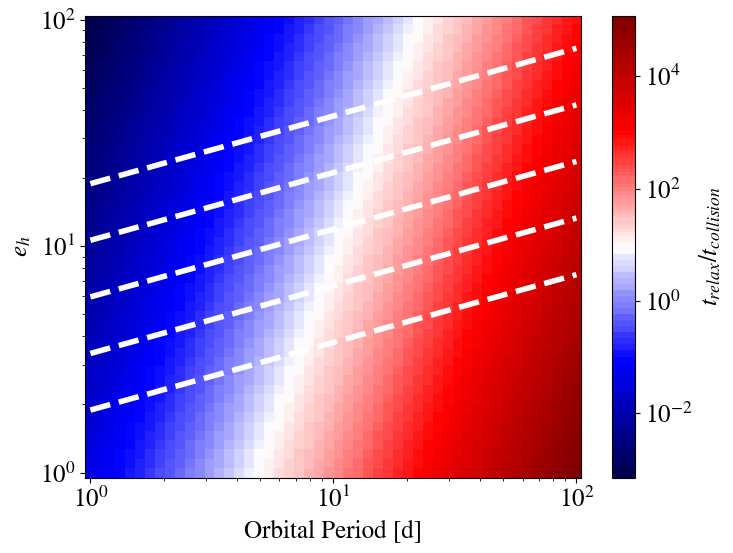
\includegraphics[width=0.5\textwidth]{figures/timescales.png}
    \caption{The ratio between the two-body relaxation and collision
      timescale for a population of equal-mass planetesimals with an
      internal density of 3 g cm$^{-3}$ and an eccentricity dispersion
      characterized by $e_h$, where $e_h = 1$ is the boundary between
      shear and dispersion dominated encounters. Only in regions where $t_{relax} \ll t_{coll}$ can the velocity distribution respond to changes in the mass of the bodies such that oligarchic growth can operate. This condition is no longer satisfied for a dynamically hot disk at sufficiently short orbital periods.\label{fig:timescales}}
\end{center}
\end{figure}

\subsection{Planetesimal Size and Extent of Hill Sphere}\label{sec:sizeandhill}

In the formalism described above, the mass and velocity distribution of the bodies are both a function of time. Due to the interdependence of these quantities, it is not clear whether the timescales for gravitational scattering and growth will remain proportional as the oligarchs develop. In the case of many studies of planetesimal accretion in the solar system (cite examples), the $t_{relax} \ll t_{coll}$ condition must remain true, otherwise runaway growth would have continued until all of the planetesimals were consumed. However, it isn't immediately clear what will happen if the system begins in a state where $t_{coll} \ll t_{relax}$.

An insight into the expected behavior in this regime can be gained by
defining the dimensionless parameter $\alpha$, which is the ratio
between the physical size of a body and it's Hill radius, $r_{h}$:
\begin{equation}\label{eq:alpha}
	\alpha = \frac{r_{pl}}{r_{h}} = \frac{1}{a} \left( \frac{9 M_{\star}}{4 \pi \rho_{pl}} \right)^{1/3},
\end{equation}
where $a$ is the semimajor axis of the body and $\rho_{pl}$ is its bulk density. Assuming a fixed bulk density as bodies collide and grow, and that no large-scale migration occurs, the scaling of both $r_{pl}$ and $r_{h}$ with $m_{pl}^{1/3}$ means that $\alpha$ will be constant with time. For a composition of ice and rock, $\alpha$ is small for any populated region of the solar system ($\alpha \sim 10^{-2}$ for Earth and $\alpha \sim 10^{-4}$ in the Kuiper belt). As one moves close to the star $\alpha$ becomes larger than 1, which implies that the physical extent of a body exceeds its Hill sphere. (also mention that hill sphere size independent of velocity for small eccentricity)

The size of $\alpha$ controls the relative importance of gravitational scattering and collisions in driving the evolution of the planetesimal disk. In the case that $\alpha$ is small, most close encounters will result in a gravitational interaction only, moving the system toward a state of relaxation. If, however, the Hill sphere is largely filled by the body itself, these same encounters will instead drive evolution of the masses. Because $\alpha$ is independent of time, the innermost region of the planetesimal disk, where collisions dominate over scattering events, should remain that way.

We also introduce a second dimensionless quantity, which relates the physical size of the bodies to the velocity state of the system
\begin{equation}\label{eq:beta}
	\beta = \frac{r_{pl}}{r_{g}}.
\end{equation}
where $r_{g} = G m_{pl} / v^{2}$ is the gravitational radius of a body. Encounters between bodies inside of a distance of $r_{g}$ result in significant deflections of their trajectories. It should be noted that the gravitational focusing enhancement factor $v^{2}/v_{esc}^{2}$ is equal to 1 for $\beta = 1$. In the case where $r_{g}$ is smaller than the size of a planetesimal, the gravitational focusing enhancement factor will be between 0 and 1.

These scaling considerations motivate the range of parameters in the
following numerical experiments as we explore the different regimes.

\section{Numerical Methods}\label{sec:methods}

We use the tree-based N-body code {\sc ChaNGa}\footnote{A public version of {\sc ChaNGa} can be downloaded from \url{http://www-hpcc.astro.washington.edu/tools/ChaNGa.html}} to model the gravitational and collisional evolution of planetesimals at short orbital periods (where $\alpha$ is large). {\sc ChaNGa} is written using the {\sc CHARM++} parallel programming language and has been shown to perform well on up to half a million processors \citep{menon15} and can follow the evolution of gravitationally interacting swarms of up to billions of particles. Using a modified Barnes-Hut tree with hexadecapole expansions of the moments to approximate forces, {\sc ChaNGa} integrates the equations of motion using a kick-drift-kick leapfrog scheme. For all of the simulations presented in this paper, we use a node opening criteria of $\theta_{BH}$ = 0.7. Additional information about the code is available in \citep{jetley08,menon15}.

Using the neighbor-finding algorithm in {\sc ChaNGa}, originally
designed for SPH calculations, we have recently implemented a solid
body collision module in the code.  This work is largely based on the
solid-body collision implementation in {\sc PKDGRAV}, which is
described in \citet{richardson94} and \citet{richardson00}. To
summarize, imminent collisions are detected during the ``drift'' phase
by extrapolating positions of bodies forward in time, using the
velocity calculated at the opening ``kick''. For each body, any
neighboring particles which fall within a search ball of radius
$2 \Delta T v + 2 r_{pl}$, where $\Delta T$ is the current timestep size
for the particle and $v$ is magnitude of its heliocentric velocity,
 are tested for an imminent collision. In the case that
a collision is detected, the particles are merged into a single larger
body, which is given the center of mass position and velocity of the
two children. Resolving a collision can produce another imminent
collision, so collisions are handled one-by-one and another full
collision check is run after the previous event is resolved. For a
more detailed description of the collision module in {\sc ChaNGa}, see
\citep{wallace19}.
Particles are advanced in time on individual timesteps chosen as a
power of two of a base timestep.  The timestep for an individual
particle is based on an estimate of the gravitational dynamical time
determined by the minimum of $\sqrt{d_{node}^3/(G(M_{node} + m_{pl}))}$
across all nodes in the tree that are accepted by the Barnes-Hut
opening criterion.  Here $d_{node}$ is the distance from the
planetesimal to the center of mass of the tree node and $M_{node}$ is
the total mass of the tree node.  For nearby particles $M_{node}$ is
replaced with the mass of the nearby particle.

\section{Narrow Annulus Simulations}\label{sec:narrow}

We begin by presenting a parameter study of planetesimal accretion,
motivated by two questions raised in section \ref{sec:theory}. 1) Does
runaway growth still operate when the condition that $v \ll v_{esc}$
is not satisfied? 2) How does planetesimal accretion proceed when the planetesimals themselves occupy a significant fraction of their Hill spheres?

To answer these questions, we run a series of simulations in which a
narrow annulus of planetesimals orbits a star. The values of $\alpha$
and $\beta$ are varied individually. 4000 planetesimals with
individual masses of $5 \times 10^{23}$ g are placed with semimajor
axes randomly drawn between 0.95 and 1.05 AU about a 1 $M_{\odot}$
star. The argument of perihelion $\omega$, longitude of ascending node
$\Omega$, and mean anomaly M for each body is drawn from a uniform
distribution $\in [0, 2 \pi)$. The inclinations and eccentricities are drawn
from a Rayleigh distribution with
$\left< i^{2} \right> = 1/2 \left< e^{2} \right>$ \citep{ida93a}.

In the ``fiducial'' case, we give the bodies a bulk density of 3 g
cm$^{-3}$, and $\left< e^{2} \right>^{1/2} = 4 e_{h}$, which corresponds to $\alpha = 3.6 \times 10^{-2}$ and $\beta = 3.4 \times 10^{-3}$. These parameters are chosen to match the initial conditions of \citet{kokubo98}, which gave rise to oligarchic growth. To vary the value of $\alpha$, we alter the bulk density of the particles. In the high-$\alpha$ case, the bulk density is reduced by a factor of $\sim$ 7100, which produces $\alpha = 1$. To vary $\beta$, the eccentricity dispersion is increased. For the high-$\beta$ case, $\left< e^{2} \right>^{1/2}$ is increased to $1500 e_{h}$, which corresponds to $\beta = 15,000$.

In all cases, the simulations are evolved with a base timestep of 1.7
days, which corresponds to 3\% of an orbital dynamical time
$\sqrt{a^3/G M_{*}}$. Due to the vastly differing growth timescales in
each case, a simulation is stopped when the growth of the most massive
body flattens out. In figure \ref{fig:alpha_beta}, we show the a-e
distribution of bodies in the initial (blue) and final (orange)
snapshots from each of the 4 simulations. The size of the points
indicates the relative masses of the bodies. Only in the case of small
$\alpha$ does a residual population of dynamically hot planetesimals
develop. The lack of high eccentricity planetesimals in the large
$\alpha$ case suggests that most encounters result in accretion
instead of scattering. In the case of large $\beta$, the protoplanets
and remaining planetesimals end up in a dynamically cool state,
compared with the initial conditions. This is due to kinetic energy 
being lost as particles inelastically collide. One final point to note 
is the difference between eccentricities of the protoplanets in the 
large $\alpha$, large $\beta$ and the small $\alpha$,
large $\beta$ case. The dynamically cooler result of the latter case
is likely due to the dominant role that inelastic collisions play here.

In figure \ref{fig:alpha_beta_mass}, we show the mass distribution of bodies from the final snapshot in each of the four cases. In addition to leaving fewer residual planetesimals, the large $\alpha$ simulations produce significantly larger embryos. Despite the vastly different encounter velocities of each population of bodies, the initial size of $\beta$ (so long as bodies remain in the dispersion-dominated regime) appears to have no significant effect on the final distribution of masses.

To investigate whether any of these planetesimal rings underwent
runaway growth, we examine the time evolution of the maximum and mean
masses in each simulation. The ratio $m_{max}/\left< m \right>$ is plotted
in figure \ref{fig:alpha_beta_evo}. On this plot, a positive slope
indicates that the maximum and mean masses are diverging (i.e.
the growth rate is accelerating with mass), which is
evident for every case we have tested. Even with a large
$\beta$, which means that the effective collision cross section is
very near the geometric value, runaway growth still appears to
operate. The ubiquity of the early positive trends in this figure indicates
that, as bodies collide and grow the
relative difference in gravitational focusing factors between bodies
is what drives the system towards runaway
growth. Although larger encounter velocities lengthen the growth
timescales, this mode of growth appears to be inevitable, so long as
gravity is the dominant force in the system. For the large $\alpha$
cases, the curves in this figure eventually turn over and begin to decline.
Upon inspecting the simulation snapshots, we find that this trend is
driven by an increase in the average mass as the planetesimal population
becomes depleted. One should expect that the same thing will eventually
occur for small $\alpha$, although many more timesteps are required to
begin to run out of planetesimals.

Additionally, these results suggest that the value of $\alpha$, which is a function of only the initial conditions (the physical and Hill radius both scale with $M^{1/3}$, so $\alpha$ stays constant as bodies grow), controls the qualitative outcome of accretion. Across most of a planet-forming disk, $\alpha$ is small, and frequent gravitational encounters between the growing bodies will facilitate oligarchic growth. In the dispersion-dominated regime, close encounters drive the stirring between planetesimals and embryos \citep{weidenschilling89, ida90}. When $\alpha$ is large, the Hill sphere of a body is no longer mostly empty space, and close encounters that would otherwise result in stirring instead result in accretion. In this regime, we observe that runaway growth still commences, but nearly all of the planetesimals are swept up by the forming protoplanets, rather than being scattered onto higher eccentricity orbits, where they would otherwise remain as a remnant of the early stages of planet formation \citep{kokubo98, kokubo00}.

% Additional idea: run a simulation with an oligarch embedded in a disk of planetesimals for large and small alpha. Allow oligarch and planetesimals to collide. What does the eccentricity evolution of the oligarch look like in each case?

% One thing im still not clear on: In dispersion dominated regime, distant encounters are what drive VS + DF. These encounters happen well outside of the Hill sphere. Why does it appear to matter if the geometric cross section fills a significant chunk of the hill sphere? And why doesn't the velocity dispersion (beta large or small) appear to matter?

% According to Ida 1990, 'distant encounters are not important' (but viscous stirring timescale can be described by Chandresehkar time). Also Weidenschilling 1989. This is also consistent with Goldreich 2004. So then why does the Armitage book describe viscous stirring in terms of distant encounters (b > b_min)?

% Wetherill + Stewart 1989, Ohtsuki 1990, Spaute 1991 find that runaway growth happens when velocity decreases with mass. Is that what we're seeing at high alpha?

\begin{table}
\caption{Summary of Full Disk Simulations Run}
\begin{tabular}{llllll} \hline \hline
Name    & $m_{pl}^{a}$ & $N_{pl}^{b}$ & $A^{c}$ & $\alpha^{d}$ &  \\ \hline
fdHi                 & $5 \times 10^{22}$ & 903,687 & 100                                                         & 1.5                              &   \\
fdHiShallow    & $5 \times 10^{22}$ & 903,687 & 100                                                        & 0.5                              &   \\
fdHiSteep       & $5 \times 10^{22}$ & 903,687 & 100                                                         & 2.5                              &   \\
fdLo                & $5 \times 10^{22}$ & 45,185    & 1                                                             & 1.5                              &   \\ \hline
\end{tabular}
\begin{flushleft}
\textsc{Note} \\ {$^a$ Planetesimal mass [g] \\
		       $^b$ Number of planetesimals \\
		       $^c$ Solid surface density normalization (relative to MMSN) \\
		       $^d$ Solid surface density power law index } \\
\end{flushleft}
\label{tab:sims}
\end{table}

\section{Full Disk Simulation}\label{sec:fulldisk}

\subsection{Initial Conditions}

Motivated by the dependence of accretion modes on $\alpha$,
we next investigate whether this highly efficient, non-oligarchic
growth should be expected to operate near the innermost regions of a typical planet-forming
disk. Given that N-body simulations of short-period terrestrial planet formation 
typically begin with a chain of neatly-spaced, isolation mass 
(see \citet{kokubo00} eq. 20) protoplanets, it is pertinent to determine 
whether the high $\alpha$ growth mode we revealed
in the previous section invalidates this choice of initial conditions.

Given the dearth of short-period terrestrial planets observed around M stars (e.g. TRAPPIST-1), we chose to model the evolution of a series of wide planetesimal disks, which span from 1 to 100 days in orbital period, orbiting a late-type M star of mass 0.08 $M_{\odot}$. For a population of planetesimals with a bulk density of 3 g cm$^{-3}$, this orbital period range corresponds to $\alpha \in (0.7, 0.05)$. By simultaneously modeling a broad range of orbital periods, we can determine the critical value of $\alpha$ that divides these two modes of accretion, and also explore how the oligarchic/non-oligarchic accretion boundary affects the resulting distribution of protoplanets.

Four wide-disk simulations are run in total (see table \ref{tab:sims}). In each case, the solid surface density follows a power law profile
\begin{equation}
	\Sigma(r) = \left( \frac{M_{*}}{M_{\odot}} \right) A \Sigma_{\mathrm{MMSN}} \left( \frac{r}{1 \mathrm{AU}} \right)^{-\delta},
\end{equation}
where $M_{*}$ is the mass of the central star, $\Sigma_{MMSN} = 10$ g cm$^{-2}$ is surface density of the minimum-mass solar nebula \citep{hayashi81} at 1 AU, and $A$ is an enhancement factor. In the first case (fdHi), we model a disk that follows a MMSN power law slope, with the overall normalization enhanced by a factor of 100. This choice of normalization for the solid surface density profile appears necessary in order to reproduce many observed short period terrestrial worlds in-situ \citep{hansen12}. Additionally, we vary the power law index (fdHiShallow, fdHiSteep) and overall normalization (fdLo) of $\Sigma(r)$.

In all cases, the eccentricities and inclinations of the bodies are randomly drawn from a Rayleigh distribution, with $\left< e^{2} \right>^{1/2} = 2\left<i^{2} \right>^{1/2} = e_{eq}$. The value of $e_{eq}$ is chosen such that the timescales for viscous stirring and aerodynamic gas drag on the planetesimals are in equilibrium. The viscous stirring timescale is given by \citet{ida93} as

\begin{equation}\label{eq:vs_timescale}
    \tau_{vs}  = \frac{\left< e^2 \right>}{d \left< e^2 \right> / dt} \approx \frac{1}{40}\left(\frac{\Omega^{2} a^{3}}{2 G m_{pl}}\right)^{2} \frac{4 m_{pl} \langle e^{2} \rangle^{2}}{\Sigma a^{2} \Omega},
\end{equation}

\noindent where $\Omega$, $a$ and $e$ are the orbital frequencies, semimajor axes and eccentricities of the individual planetesimals. In the Stokes regime, the gas drag timescale is given by \citet{adachi76} as

\begin{equation}\label{eq:ts_stokes}
    t_{s} = \frac{2 m_{pl}}{C_{D} \pi r_{pl}^{2} \rho_{g} v_{g}},
\end{equation}

\noindent where $C_{D}$ is a drag coefficient of order unity, $\rho_{g}$ is the local gas volume density and $v_{g}$ is the headwind velocity of the gas experienced by the planetesimal. The local gas volume density is given by

\begin{equation}\label{eq:rho_gas}
	\rho_{g} = \frac{\Sigma_{g}}{\sqrt{2 \pi} h_{g} \exp\left[ -z^{2} / \left( 2 h_{g}^{2} \right) \right]},
\end{equation}

\noindent where $\Sigma_{g}$ is the gas surface density (taken to be
240 times the solid surface density), $h_{g} = c_{s} / \Omega$ is the local gas scale height and $z$ is the height above the disk midplane. The sound speed profile is given by $c_{s} = \sqrt{k_{B} T(r) / \left( \mu m_{H} \right)}$, where $k_{B}$ is Boltzmann's constant, $T(r) = T_{0} r^{-Q}$, $\mu = 2.34$ and $m_{h}$ is the mass of a hydrogen atom. For a protoplanetary disk around a typical M star, $T_{0} = 148$ K and $Q$ = 0.58 \citep{andrews05}.

Finally, the headwind velocity of the gas, due to the fact that the gas disk is pressure supported, is given by

\begin{equation}\label{eq:v_gas}
	v_{g} = v_{k} \left[ 1 - \sqrt{ Q c_{s}^2 / v_{k}^2} \right],
\end{equation}

\noindent where $v_{k}$ is the local Keplerian velocity. As in section
\ref{sec:narrow}, the argument of perihelion $\omega$, longitude of
ascending node $\Omega$, and mean anomaly M for the planetesimals are drawn from a uniform distribution $\in [0, 2 \pi)$.

\subsection{Gas Drag Force}

In addition to the mutual gravitational forces, a Stokes drag force from to the gas disk is applied to each particle, following the prescription described in section 2.2.1 of \citet{morishima10}.

\subsection{Timestepping Criterion}

In the case of the fdHi simulation, there are nearly 1 million
particles, whose orbital periods vary by two orders of magnitude. Because the
interaction timescales near the inner edge of the
disk are exceedingly short, a fixed timestep size would required a prohibitively large
number of steps to follow planetesimal growth throughout the entire
disk. For this reason, we use a multi-tiered timestepping scheme, in
which particles are placed onto the nearest power of two timestep
based on their most recently calculated gravitational
acceleration. \footnote{This scheme is used on almost all works using ChaNGa,
and is common among large-scale simulation codes.}

This more efficient scheme introduces two issues, however. Firstly,
momentum is not completely conserved when bodies switch timesteps. The
error introduced becomes particularly severe for a particle on an
eccentric Keplerian orbit, whose perihelion and aphelion distances
straddle a timestep boundary. For a large collection of particles,
this problem manifests itself as the development of a V-shaped gap in the semimajor axis-eccentricity plane, which is centered on the boundary itself. To correct this problem, we introduce a slightly modified timestepping criterion, which is based on the expected gravitational acceleration of the particle at pericenter. Only in the case of a close encounter with another planetesimal (in which the acceleration is no longer dominated by the star) is the timestep allowed to reduce based on the original criterion.

A second issue is introduced when two particles on different timesteps undergo a collision. As in the previous case, momentum is not completely conserved because the most recent `kick' steps did not happen simultaneously for these bodies. Early in the simulation, we find that runaway growth tends to initiate at the timestep boundaries. This issue carries itself forward through the embryo formation phase, and protoplanets tend to form at the boundaries. To correct this issue, we ignore collisions between bodies on different timesteps early in the simulation. We find that preventing multi-timestep collisions until after the maximum mass grows by a factor of 10 prevents any artifacts from developing at the timestep boundaries, while also minimizing the number of `skipped' collisions\footnote{In the case of fdHi, only about 20 collisions out of an eventual 900,000 are ignored.}. 

\subsection{Results}

\begin{table}
\caption{Final Properties of Full Disk Simulations}
\begin{tabular}{lllll} \hline \hline
Name     & $M_{PP}^a$ & $T_{int}^b$ & $T_{int 1}^c$ &  \\ \hline
fdHi                 &  1.00                                                         & 456                              & 16,377  &  \\
fdHiShallow    &  1.19                                                        & 456                              & 16,377  &  \\
fdHiSteep       &  1.08                                                         & 456                              & 16,377 &  \\
fdLo                &  1.77 $\times 10^{-3}$                                  & 3,713                              & 133,651 &  \\ \hline
\end{tabular}
\label{tab:sim_properties}
\begin{flushleft}
\textsc{Note} \\ {$^a$ Maximum protoplanet mass [$M_{earth}$] \\
		       $^b$ Integration time [yr] \\
		       $^c$ Rescaled integration time [yr]} \\
\end{flushleft}
\end{table}

The timescales for embryo formation depend on
the chosen surface density profile, along with the local orbital
timescale. Protoplanets form first at the inner edge of the disk,
where the dynamical timescales are short. Growth proceeds in an
inside-out fashion, with the outermost regions of the disk completing
the protoplanet assembly phase last. This radial timescale dependence is not typically
accounted for in planet formation simulations\footnote{Instead, the innermost protoplanets 
patiently `wait' for this phase of evolution to complete everywhere in the disk}, and appears to be an
important component to forming realistic solar system analogs
\citep{clement20}. As with the narrow annulus simulations, we stop the
integration once the masses of protoplanets in the outermost region of
the disk reach a steady value. In table \ref{tab:sim_properties}, we
summarize the outcomes of the four ``full disk'' cases.

We show the final state of the ``fdHi'' simulation in figure \ref{fig:fulldisk_e_m}. In the top panel,
the initial (contours) and final (points) state of the simulation is shown in the orbital period-eccentricity plane. The size of the points indicates the relative mass of the bodies. In the bottom panel, the mass of the largest bodies is shown as a function of orbital period. The solid curves indicate the isolation mass,
\begin{equation}\label{eq:iso}
	M_{iso} = \left[ \frac{\left( 2 \pi a^2 \Sigma \tilde{b} \right)^3}{3 M_{*}} \right]^{1/2},
\end{equation}
where $\tilde{b}$ is the size of the feeding zone in units
of Hill radii. For two bodies on circular, non-inclined orbits,  $\tilde{b} = 2
\sqrt{3}$ is the smallest orbital separation that produces a non-negative Jacobi energy
and permits a close encounter (see \citet{naka88}).
The isolation mass is plotted in blue and orange for these two values of $\tilde{b}$, respectively.

A qualitative shift in the protoplanet and planetesimal distribution is visible at $\sim$ 60 days. Interior to this location, there are very few remaining planetesimals and the embryos formed are noticeably more massive. Protoplanets in this region appear to closely follow the isolation mass curve for $\tilde{b} = 10$. Exterior to the boundary, the residual planetesimal population is much more pristine, and protoplanets more closely follow the $\tilde{b} = 2 \sqrt{3}$ curve. This suggests that the transition between the low $\alpha$ and high $\alpha$ accretion modes seen in section \ref{sec:narrow} happens near this location.

In section \ref{sec:narrow}, we postulated that the increased importance of inelastic damping in the inner, non-oligarchic growth region of the disk should lower the overall eccentricity of the protoplanets there. This behavior is not immediately apparent in the top panel of figure \ref{fig:fulldisk_e_m}. There are, however, a couple of factors in the wide disk simulations that could make this extra dynamical cooling mechanism difficult to see. Firstly, the initial eccentricity distributions of the inner and outer disk are different because of the dependence of the viscous stirring and gas drag timescales on orbital period. Additionally, the protoplanet formation timescales for the inner and outer disk are vastly different, rendering a comparison between these regions at the same moment in time inappropriate.

%In figure (removed), we show $\alpha$ (left axis) and the fraction of remaining planetesimals (right axis) as a function of orbital period. Here, the fraction of remaining planetesimals is measured by dividing the disk into 15 semimajor axis bins and using the profile function in {\sc pynbody} to measure the total solid surface density $\Sigma$ in each of those bins, and also the planetesimal surface density $\sigma$. Here, a planetesimal is defined to any body with $m < 10 m_{pl}$. Exterior to 60 days in orbital period, $\sigma/\Sigma$ sharply increases, indicating that the highly efficient accretion mode seen previously does not operate here. As can be seen from the plot, the accretion boundary roughly corresponds to $\alpha = 0.1$.
% This figure could be turned into a few sentences in the text.

% A mystery: what's so special about alpha = 0.1?

To ensure that the boundary seen near 60 days in orbital period is not
simply a transient product of the inside-out growth throughout the
disk, we examine the time evolution of $\sigma/\Sigma$ at multiple
locations. In figure \ref{fig:pl_frac_time}, the value of
$\sigma/\Sigma$ is plotted as a function of time in 10 orbital period
bins, each with a width of 10 days.
Bins interior to 60 days are indicated with a dashed line, while those exterior are indicated with a solid line. In all radial bins, the planetesimal surface density is approaching an asymptotic value. In the inner disk, this value asymptotes to zero as the planetesimal population completely depletes. In the outer disk, dynamical friction between the embryos and planetesimals eventually throttles subsequent accretion and leaves $\sim$ 10 to 20 percent of the mass surface density as planetesimals.

% Another important point: the accretion boundary doesn't move as we change surface density (how does t_relax and t_coll scale with sigma?). More evidence that it just depends on alpha(r)

\begin{figure*}
\begin{center}
    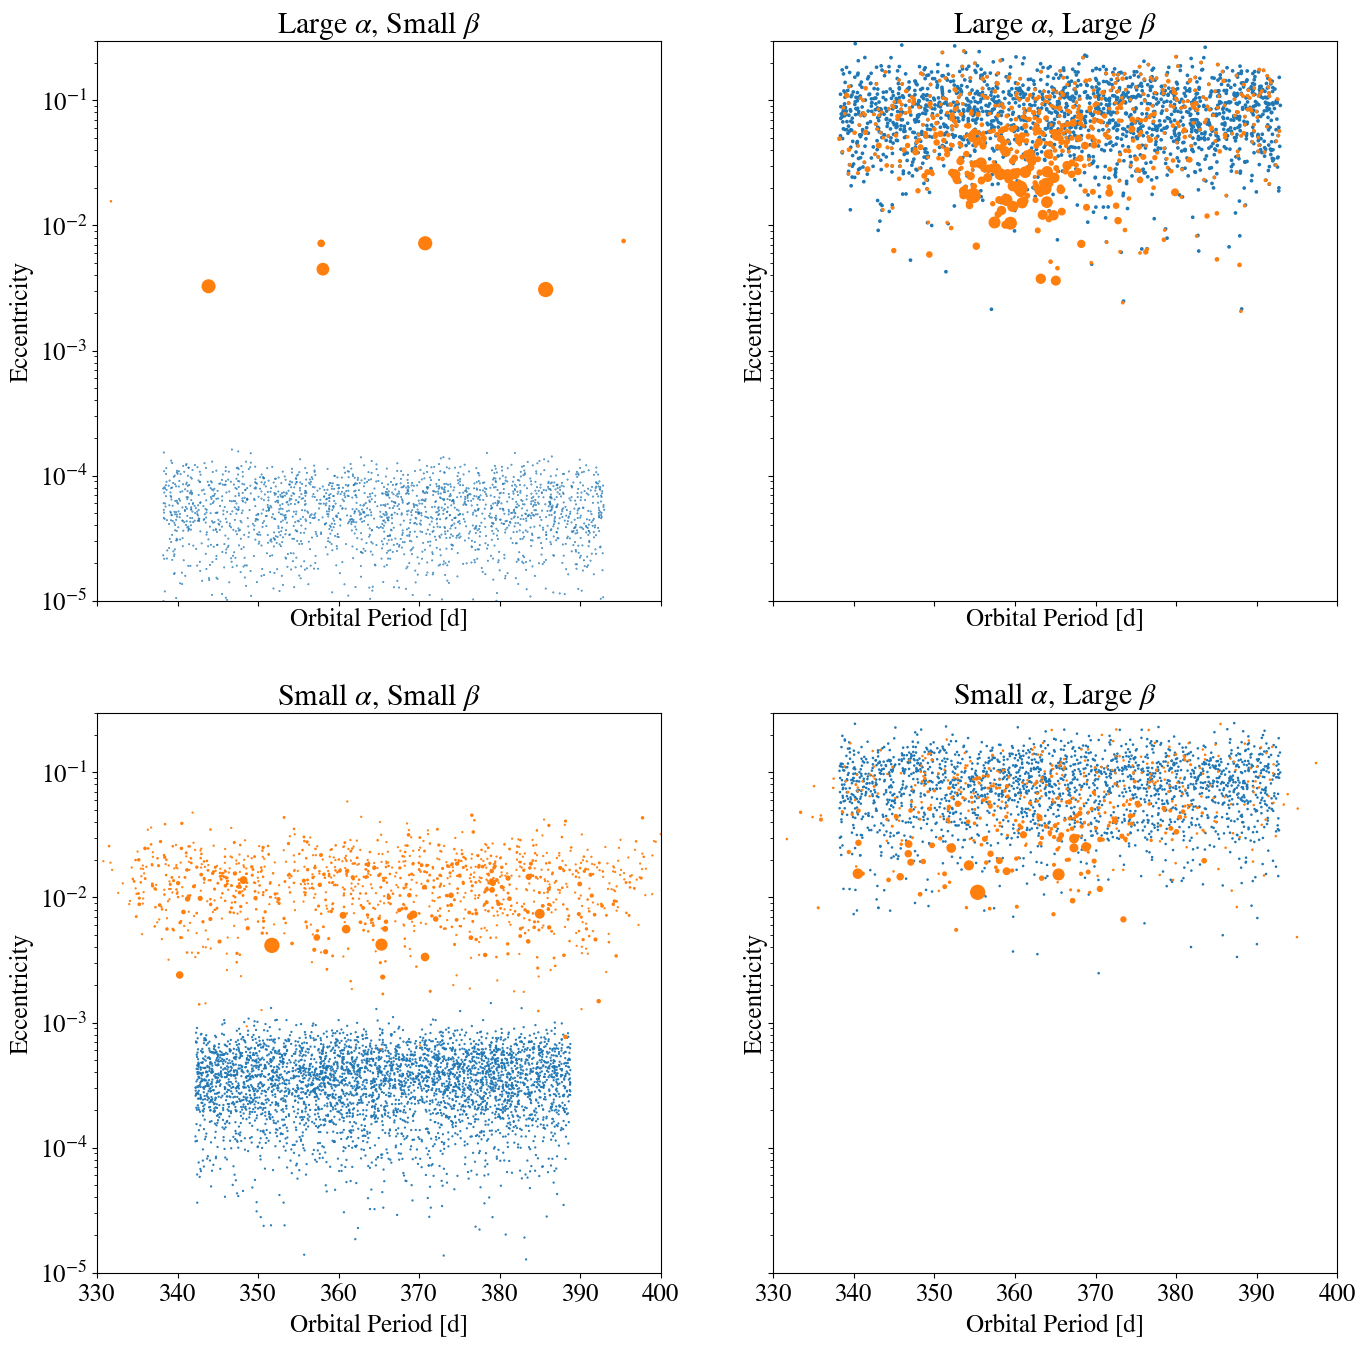
\includegraphics[width=\textwidth]{figures/alpha_beta.png}
    \caption{The initial (blue) and final (orange) states of the simulations described in section \ref{sec:narrow}. Relative masses of the bodies are indicated by point size. In the case of large $\alpha$, almost no residual planetesimal population remains. Regardless of the initial choice of $\beta$, the protoplanets that form attain similar eccentricities. \label{fig:alpha_beta}}
\end{center}
\end{figure*}

\begin{figure}
\begin{center}
    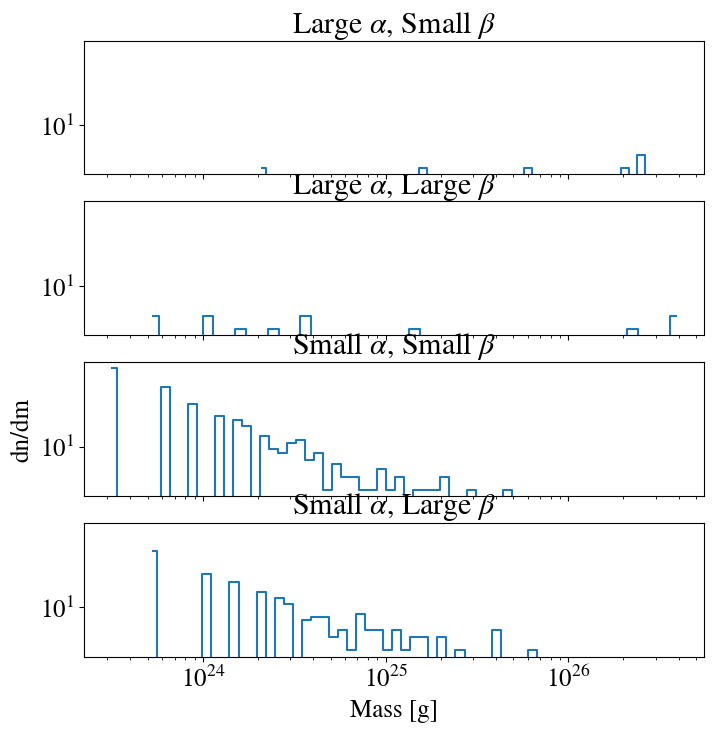
\includegraphics[width=0.5\textwidth]{figures/alpha_beta_mass.png}
    \caption{The final state of the mass distribution for the
      simulations described in section \ref{sec:narrow}. For small
      $\alpha$, a few embryos form alongside a power law tail of
      planetesimals. For larger values of $\alpha$, the mass
      distribution takes on a more uniform form. As in the previous figure, the initial choice of $\beta$ does not appear to have any meaningful impact on the end result.\label{fig:alpha_beta_mass}}
\end{center}
\end{figure}

\begin{figure}
\begin{center}
    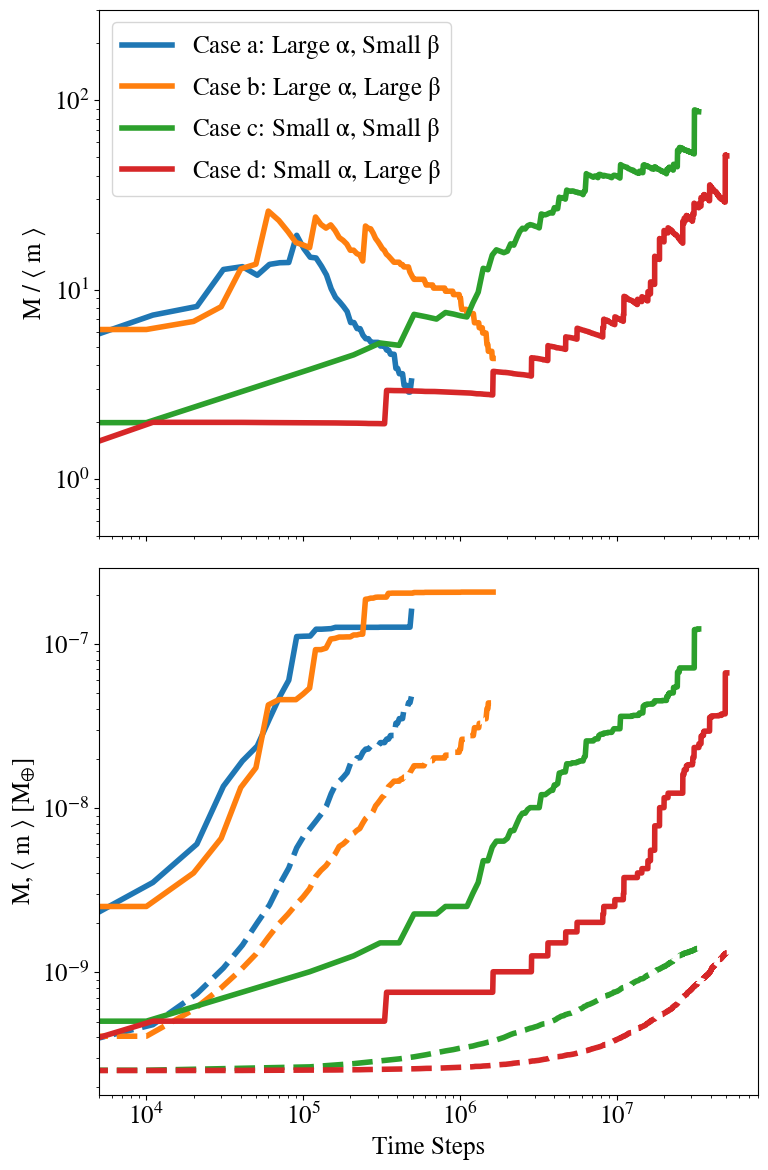
\includegraphics[width=0.5\textwidth]{figures/alpha_beta_evo.png}
    \caption{The evolution of the ratio between the maximum and mean mass for the four simulations presented in section \ref{sec:narrow}. The runaway growth phase can be identified by a positive slope in this ratio. For all values of $\alpha$, an increase in $\beta$ has the effect of delaying the growth of the embryos.\label{fig:alpha_beta_evo}}
\end{center}
\end{figure}

% show 4 panel plot of period-e distribution for large, small alpha and beta
% show that runaway growth still operates for large beta

\begin{figure}
\begin{center}
    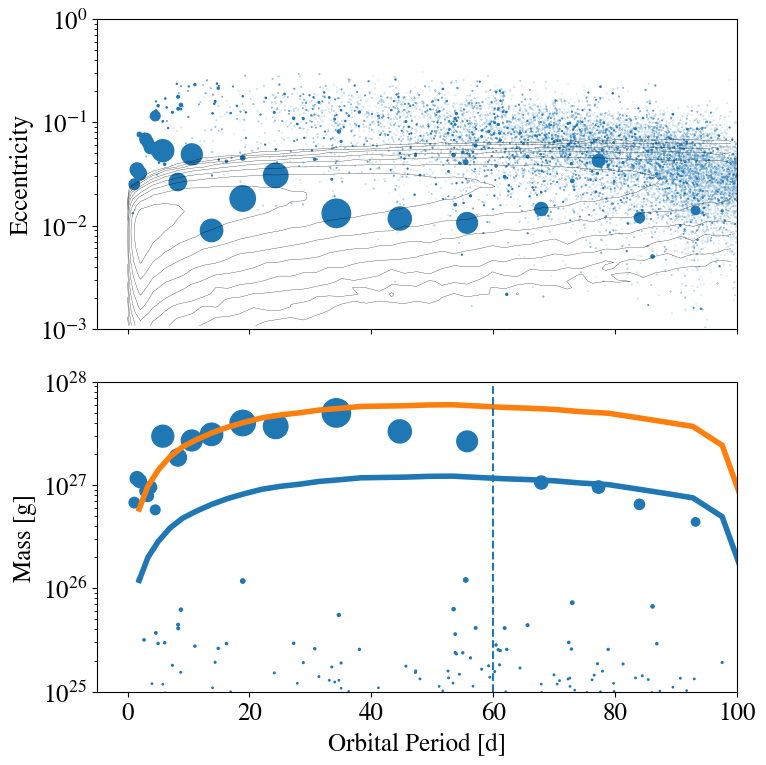
\includegraphics[width=0.5\textwidth]{figures/fulldisk_e_m.png}
    \caption{The final state of the fdHi simulation. In the top panel,
      the contours denote the initial period-eccentricity distribution
      of the planetesimals. Point sizes indicate the relative masses
      of bodies. In the bottom panel, the solid line indicates the
      isolation mass for $\tilde{b} = 2 \sqrt{3}$. The vertical dashed line marks the approximate location of the accretion mode boundary. For $P_{orb} < 60$ days, the high $\alpha$ accretion mode produces embryos that exceed the isolation mass.\label{fig:fulldisk_e_m}}
\end{center}
\end{figure}

\begin{figure}
\begin{center}
    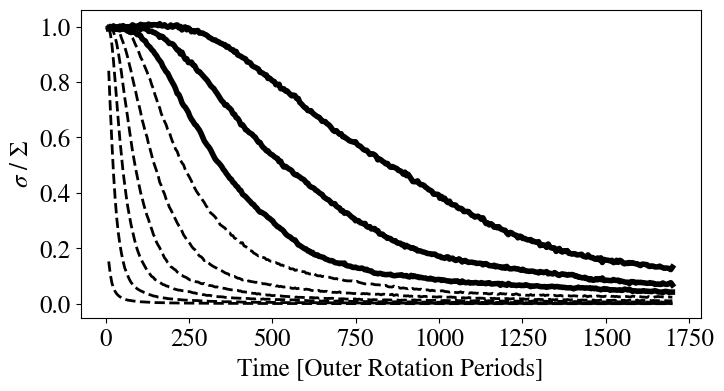
\includegraphics[width=0.5\textwidth]{figures/pl_frac_time.png}
    \caption{The time evolution of the planetesimal surface density (in units of the total solid surface density) in the fdHi simulation. Each curve represents a radial slice of the disk. The innermost region evolves the quickest, and is therefore represented by the lowest curve. The dashed lines indicate radial zones interior to the 60 day orbital period boundary.\label{fig:pl_frac_time}}
\end{center}
\end{figure}

\begin{figure}
\begin{center}
    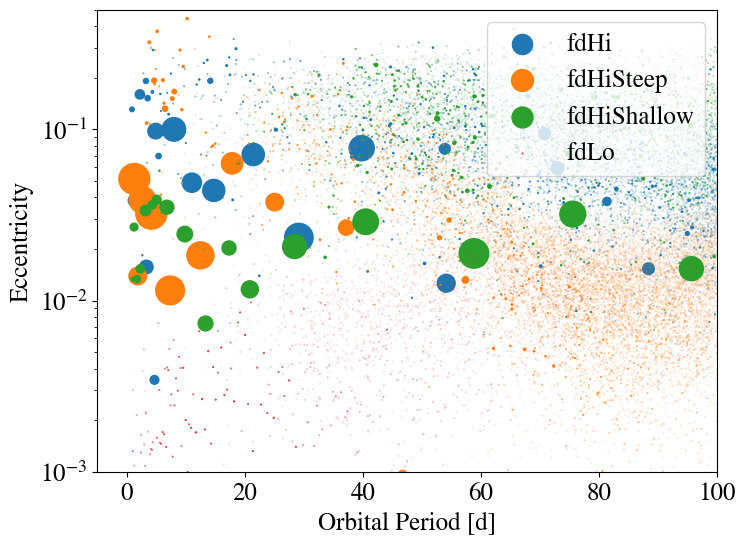
\includegraphics[width=0.5\textwidth]{figures/surfden_profiles.png}
    \caption{The final state of all simulations listed in table \ref{tab:sim_properties}. Point sizes indicate mass relative to the largest body in the fdHi simulation.\label{fig:surfden_profiles}}
\end{center}
\end{figure}

\begin{figure}
\begin{center}
    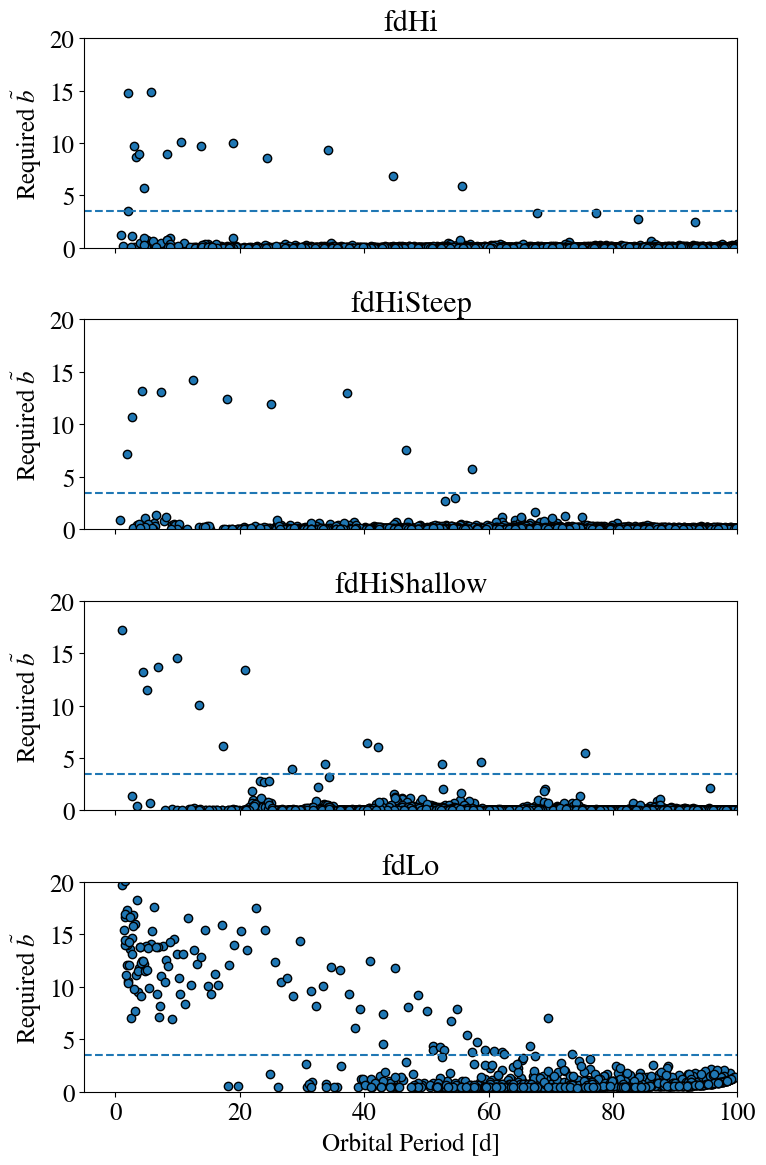
\includegraphics[width=0.5\textwidth]{figures/surfden_b.png}
    \caption{Feeding zone width (see equation \ref{eq:iso} required to produce the final masses for the protoplanets from the simulations listed in table \ref{tab:sim_properties}. The horizontal dashed line indicates $\tilde{b} = 2 \sqrt{3}$. Despite the vastly different initial solid surface density profiles, the feeding zone width reaches the circular orbit value around $\sim$ 60 days. \label{fig:surfden_b}}
\end{center}
\end{figure}

% show period-e distribution
% show show period-mass distribution, with isolation mass curve overlaid
% what about 'maximum planetary mass' from Schlichting 2014?
% show plot of period vs alpha, mass. drop in embryo mass occurs where alpha = 0.1
% also plot period vs sigma/Sigma and mass with alpha=0.1 location marked. residual planetesimal population missing interior to alpha=0.1

% does the accretion boundary always fall somewhere within the PPD, or can it lie inside the magnetic truncation radius sometimes? how does this depend on spectral type? (this is complicated, depends on radius + magnetic field strength of star, plus accretion rate of PPD)

Next, we compare the effect of varying the initial solid surface
density profile on the resulting planetesimal and embryo
distribution. The final orbital period-eccentricity state of the
particles is shown in figure \ref{fig:surfden_profiles}, with colors
and point styles indicating the different initial surface density profiles,
and with point sizes indicating the relative masses of the bodies. There is a clear trend between solid surface density at a given orbital period and the eccentricities of the remaining planetesimals. This trend is largely set by the initial conditions, as the gravitational stirring is more vigorous when bodies are packed together closely and higher eccentricities are required to produce an equilibrating aerodynamic drag force (see equations \ref{eq:vs_timescale} and \ref{eq:ts_stokes}). Despite having significantly different masses, the planetary embryos formed in each case have remarkably similar eccentricities. This is likely due to the fact that inelastic collisions play a more significant role where the solid surface density is highest, which offsets the fact that the initial bodies started off in a dynamically hotter state.

% Period vs mass for each model?
% Positive trend for trappist-1 planets, excluding a,b

In figure \ref{fig:surfden_b}, we plot the masses of the resulting protoplanets and planetesimals in all four simulations in units of $\tilde{b}$ (see equation \ref{eq:iso}). Here, we assume that each embryo has reached its isolation mass, and that differences in mass are driven by differences in the initial surface density at the embryo's current location, along with the size of its feeding zone, which is set by the dynamics relevant at that location in the disk. By plotting the derived value of $\tilde{b}$ as a function of orbital period, differences in the dynamical interactions at different locations of the disk are made more clearly visible. As mentioned previously, $\tilde{b} = 2 \sqrt{3}$ (indicated by the horizontal dashed line) carries a special significance, being the minimum feeding zone width that a body can have. In all four simulations, the feeding zone width exceeds the minimum value in the inner disk and approaches $2 \sqrt{3}$ beyond $\sim$ 60 days. The orbital periods at which this transition occurs are remarkably similar, despite the vastly different solid surface density profiles used. This similarity indicates that the boundary between accretion modes is not dependent upon the surface density profile chosen, and also supports our conclusion that planetesimal accretion is largely complete everywhere in the disk.

%In figure \ref{fig:surfden_iso}, we compare the masses of the resulting protoplanets and planetesimals in all four simulations to each other. Here, the masses are scaled by the isolation mass at the given orbital distance (see equation \ref{eq:iso}). In all four cases, the masses follow a similar trend: interior to about 60 days in orbital period, protoplanets grow to a factor of a few larger than $M_{iso}$. Exterior to this point, the protoplanet masses roughly stay near the isolation mass. Despite the drastically different solid surface density profiles used, the masses of the largest bodies in all four cases follow a similar trend with orbital period. This indicates that the highly efficient accretion mode seen at shorter orbital periods is dependent on the sizes of the individual bodies themselves, rather than how they are distributed. The transition visible near 60 days in all cases also supports our conclusion that planetesimal accretion is largely complete everywhere in the disk.

\subsection{Assembly History of Embryos}\label{sec:assembly}

Further insight into the difference between the short vs long period accretion modes can be gained by examining the merger history of the planetary embryos. Because all collisions are directly resolved by the N-body code, a direct lineage can be traced between each embryo and a set of initial planetesimals.

We begin by investigating the ``smoothness'' of the accretion events
that give rise to each embryo. Drawing from a common technique used
for cosmological simulations (citation?), we divide growth events for
a given body into ``major'' and ``minor'' mergers. Minor events are defined as any collision involving an initial planetesimal, while major events consist of any two larger bodies. In figure \ref{fig:minor_frac}, we show the total mass fraction gained by minor events as a function of mass for the 100 largest bodies at the end of fdHi. Blue dots represent bodies interior to the 60 day orbital period boundary, while red crosses indicate bodies exterior. For the outer bodies in the oligarchic growth region, we see a very weak trend between minor accretion mass fraction and total mass. Regardless of how much an embryo has grown, the initial mass planetesimals contribute about the same relative amount to its total mass. At shorter orbital periods, however, there is a somewhat stronger trend. The largest bodies in this region gain about an order of magnitude more of their mass fraction from major mergers, compared to the smallest bodies.

\begin{figure}
\begin{center}
    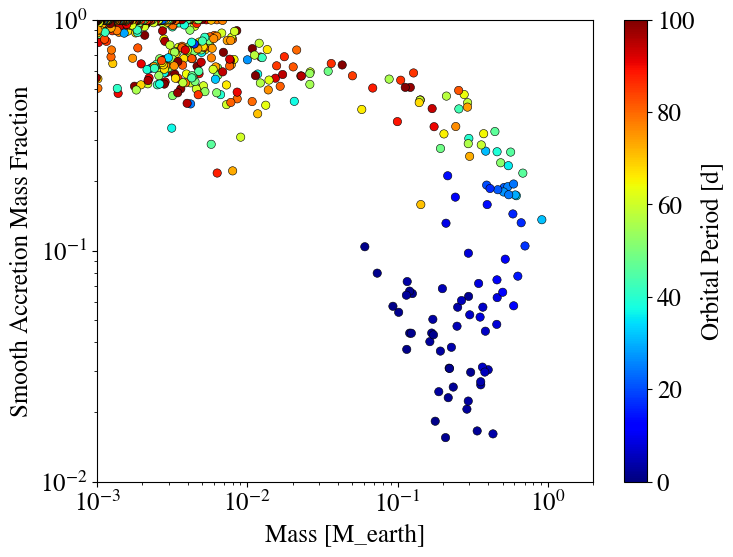
\includegraphics[width=0.5\textwidth]{figures/minor_frac.png}
    \caption{For the 100 most massive bodies at the end of the fdHi simulation, the fraction of their total mass attained through mergers with initial mass planetesimals (smooth accretion) as a function of total mass. Bodies that reside beyond the 60 day accretion boundary are shown with red crosses, while bodies interior to the boundary are shown with blue dots. For the short period bodies, there is a decreasing correlation between smooth accretion fraction and mass, which suggests that most growth occurs between equal mass bodies. For the longer period bodies in the oligarchic growth region, this trend is flat, indicating that accretion of planetesimals is important during all phases of evolution.\label{fig:minor_frac}}
\end{center}
\end{figure}

\begin{figure*}
\begin{center}
    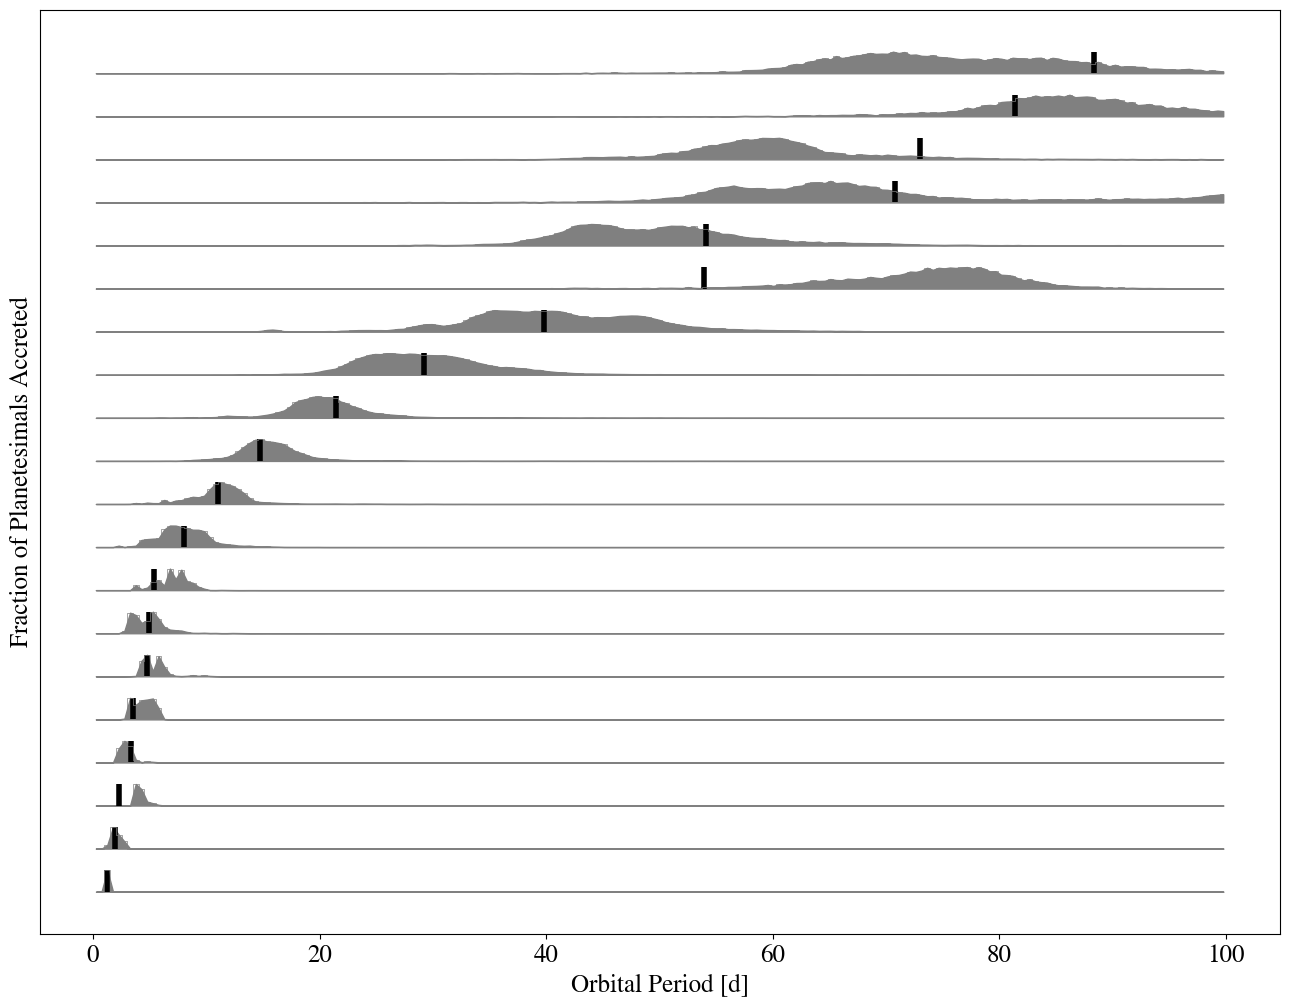
\includegraphics[width=\textwidth]{figures/acc_zones.png}
    \caption{For the 20 most massive bodies at the end of the fdHi simulation, the relative shape of the accretion zones for each body are shown. The black hash marks indicate the present position of the body. The accretion distributions indicate the initial locations of the planetesimals that were used to assemble a body, rather than the locations at which collisions with the massive body occurred.\label{fig:acc_zones}}
\end{center}
\end{figure*}

The difference in slope of the short vs.\ long period bodies in figure \ref{fig:minor_frac} indicates a difference in how the planetesimal-embryo populations interact in each region. In the long period oligarchic growth region, embryos continue to accrete planetesimals as they grow and the minor mass fraction stays mostly flat. At short period, collisions mostly occur between equal mass bodies as the embryos grow and the contribution from planetesimals becomes less significant over time. This suggests that embryo-embryo collisions are common at short period. As discussed in section \ref{sec:sizeandhill}, the importance of gravitational scattering is greatly reduced here. Without frequent gravitational interactions between the embryos and planetesimals, orbital repulsion \citep{kokubo98} and isolation of the embryos does not occur. As we showed in figure \ref{fig:surfden_iso}, the embryos formed in this region exceed the isolation mass.

Further evidence for the lack of gravitational scattering events in
the inner region can be seen in figure \ref{fig:acc_zones}. Here, we
have chosen the 20 most massive bodies from the fdHi simulation and
arranged them in order of present orbital period. The vertical black
line indicates the orbital period of each embryo. The associated
histogram for each body denotes where the planetesimals used to
construct that embryo originated in the disk. The peaks of the
histograms have all been normalized to the same value, so that the
distributions only show the relative widths and locations of the
feeding zones. Beyond the 60 day boundary, the ordering of the feeding
zones and the embryo locations become much less consistent. This
suggests that scattering events between embryos are much more common
beyond this accretion mode boundary. In the inner region of the disk,
close encounters between embryos often result in a merger, which
allows them to grow beyond the isolation mass with only a minor alteration to their orbital period. With few close encounters resulting in a scattering event, embryos are unable to move away from their birth location.

% from how far do embryos accumulate material
% do embryos migrate at all? might need to run a simulation without gas to demonstrate whether this is due to PDM
% major vs minor mergers?

\section{Simplifying Assumptions}\label{sec:assump}

\subsection{Collision Cross Section}

In all cases shown so far, the boundary between the standard
oligarchic growth and the highly-efficient short period accretion
region lies around 60 days in orbital period. The mode of accretion is
set entirely by the local value of $\alpha$, which scales with both
distance from the star and the bulk density of the planetesimals (see
equation \ref{eq:alpha}). The artificial inflation of the collision
cross section of the particles in our simulations, which is meant to
reduce the computational expense, has the side effect of reducing the
bulk densities. Because $\alpha \sim \rho_{pl}^{-1/3}$, increasing the
particle sizes by a factor of $f=6$ reduces the orbital period at which $\alpha$ has a given value by a factor of approximately 15. Therefore, one would expect the accretion boundary to lie near 5 days in orbital period for 3 g $cm^{-3}$ bodies.

Although a simulation with $f=1$ is not computationally tractable, we
can test whether the accretion boundary moves in the way we expect by
modestly changing the value of $f$. In figure \ref{fig:f6f4}, we
compare the fdHi simulation to a nearly identical run using $f=4$. In
the top panel, the embryo masses in units of the isolation mass are
shown as a function of orbital period. In the bottom panel, the value
of $\alpha$ as a function of orbital period is shown for 3 g $cm^{-3}$
bodies with an artificial radius enhancement of $f=1$, 4 and 6. The
horizontal dashed line indicates the value of alpha below which the
accretion mode switches to oligarchic growth. Comparing the top and
bottom panels, the intersection of the embryo masses and local
isolation mass matches well with the orbital period at which $\alpha
\sim 0.1$.  Also shown by the shaded region are $\alpha$ values for
realistic sized bodies with $\rho_{pl}$ between 1 and 10 g cm$^{-3}$.
% Also shown by the curved dotted lines are the $\alpha$ curves for
% realistic-sized bodies with $\rho_{pl}$ = 1, 5 and 10 g $cm^{-3}$.
In all cases, the accretion boundary still lies within the part of the disk in which solids would be expected to accumulate (citation?).

\begin{figure}
\begin{center}
    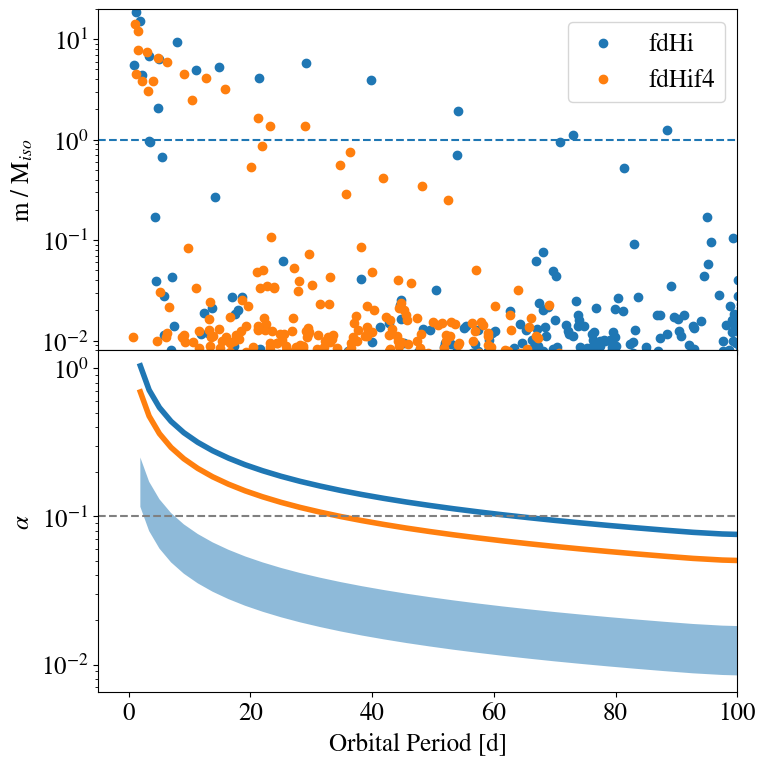
\includegraphics[width=0.5\textwidth]{figures/f6f4.png}
    \caption{In the top panel, we show the final masses of the bodies
      from the fdHi and fdHif4 simulations in units of the isolation
      mass for $\tilde{b} = 2\sqrt{3}$. The bottom panel shows the variation of $\alpha$ with orbital period for the bodies used in each case (solid curves). The orbital period at which $\alpha \simeq 0.1$ matches well with the intersection of the embryo mass distribution and isolation mass. The shaded region in the bottom panel show the values of alpha for realistic-sized ($f=1$) planetesimals with bulk densities between 10 and 1 g cm$^{-3}$.\label{fig:f6f4}}
\end{center}
\end{figure}

% compare f=4 and f=6 disk. show that the mass transition moves inwards by the correct amount as alpha changes
% how does density affect results? trappist-1 planets are 5 g/cc (agol+ 2021)

\subsection{Collision Model}

\begin{figure}
\begin{center}
    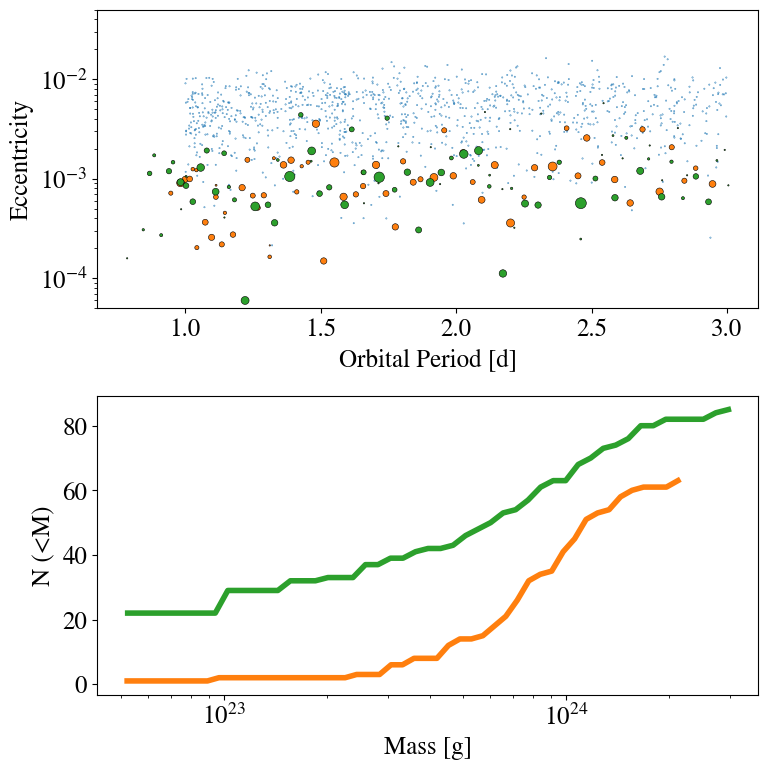
\includegraphics[width=0.5\textwidth]{figures/frag_ecc.png}
    \caption{A comparison between the innermost regions of the fdLo (orange) simulation, and a second version using a bounce-merge collision model (green). In the top panel, the period-eccentricity state of the particles is shown, with marker sizes indicating relative mass. The blue points represent the initial state of the simulations. The bottom panel compares the final masses of the bodies. \label{fig:frag_ecc}}
\end{center}
\end{figure}

\begin{figure}
\begin{center}
    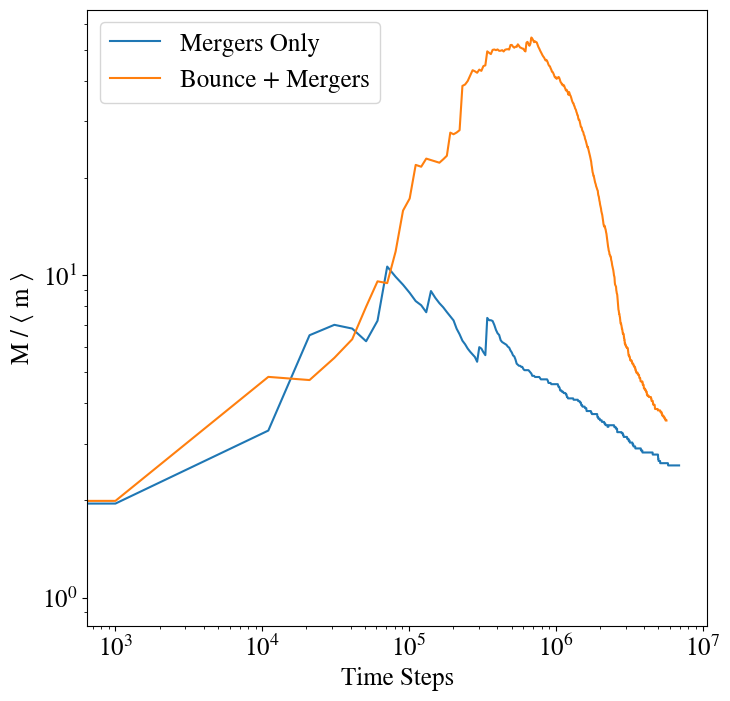
\includegraphics[width=0.5\textwidth]{figures/frag_evo.png}
    \caption{The evolution of the ratio between the maximum and mean mass of the simulations shown in figure \ref{fig:frag_ecc}. In both cases, the system first evolves through a phase of runaway growth, before the massive bodies consume the smaller bodies, driving down the mean mass. With the bounce-merge model, the mass ratio decreases later because not all collisions result in growth.\label{fig:frag_evo}}
\end{center}
\end{figure}

In the simulations presented in this work, all collisions result in a complete merging of a pair of bodies with no loss of mass or momentum. Although simple to model, this assumption of perfect accretion may result in overly efficient growth, particularly at the innermost region of the disk where encounter velocities are the largest. To handle this issue properly, semianalytic collision resolution models have been developed and implemented in N-body codes (see \citet{leinhardt12}). However, resolving collisional debris fragments using a direct approach as we have done with {\sc ChaNGa} would result in an intractably large number of particles.

To test whether a more restrictive collision model should modify our results, we present a smaller scale test using a slightly more sophisticated collision model. In this case, a collision can result in one of two outcomes: if the impact velocity is smaller than the mutual escape velocity of the colliding particles, defined as
%TRQ: I corrected this off the top of my head: CHECK!
\begin{equation}\label{eq:v_mut}
	v_{mut, esc} = \sqrt{\frac{G (m_{1} + m_{2})}{r_{1} + r_{2}}},
\end{equation}
where $m_{1}, m_{2}$ and $r_{1}, r_{2}$ are the masses and radii of
colliding particles 1 and 2, then the bodies perfectly merge. For
impact velocities larger than $v_{mut, esc}$, no mass is transferred, and the bodies undergo a completely elastic bounce. Because there is no possibility of partial accretion, this model likely restricts growth more than the model used by \citet{leinhardt12}. However, we will show below that the bounce-merge model does not meaningfully affect the outcome of the planetesimal accretion phase, and so a partial accretion model should do the same.

For the configuration of initial conditions we have chosen, the typical encounter velocity (defined by $v_{enc} = \left< e^{2} \right>^{1/2} v_{k}$, where $v_{k}$ is the local Keplerian velocity) is about 25 percent larger than $v_{mut, esc}$. Because the encounter velocities follow a Gaussian distribution, there should be some small subset of collisions that still meet the merger criteria. In addition, $v_{mut, esc}$ becomes larger as the bodies grow and the merger criteria should become easier to meet as the system evolves.

In figure \ref{fig:frag_ecc}, we show the results of two versions of the fdLo simulation, one with mergers only (shown in orange) and one with the bounce-merge model (shown in green). The blue points in the top panel show the initial conditions used for both cases. Because the bounce-merge model greatly increases the number of timesteps required, we choose to model only the innermost part of the disk to reduce the computational cost. Although the bounce-merge simulation takes much longer to reach the same phase of evolution, the resulting orbits and masses of the embryos are indistinguishable from the merger-only case.

To investigate the differences between the two collision models early in the simulations, we show the time evolution of the ratio between the maximum and mean mass in figure \ref{fig:frag_evo}. In both cases, this ratio grows at early times, which indicates that runaway growth still operates, regardless of the collision model used. In the bounce-merge case, the mass ratio peaks at a higher value, while also undergoing a longer runaway growth phase. This suggests that the mass distribution becomes much less unimodal during this growth process, but as figure \ref{fig:frag_ecc} shows, this does not affect the resulting embryos or allow for a residual planetesimal population.

%TRQ: expand on this?  Compare figure 10 histograms for the two runs?
Radial mixing appears to be enhanced by a partial collision model, along with smaller collision cross section inflation \citep{childs22}.

% show alpha, beta study again with bounce vs merge model
% mergers still happen for 'lo' simulations but not 'hi'
% this is because the eccentricity dispersion is significantly higher in the 'hi' case
% mostly because stirring rate increases with surface density
% criteria should get less restrictive as larger bodies grow, what if we turn on bounces partway thru growth process?

\subsection{Type I Migration}

What is the migration timescale for the embryos to move to the inner edge of the disk? Maybe this section isn't terribly important and should be excluded?
TRQ: I agree

\section{Summary and Discussion} \label{sec:discuss}

In this work, we have demonstrated that planetary embryo formation
operates in two distinct modes in a planet-forming disk. In the first
mode, gravitational feedback from the growing embryos heats the
remaining planetesimals and results in a dynamically cold population
of embryos with a significant amount of residual planetesimals. This
corresponds to the ``oligarchic growth'' case revealed by \citep{kokubo98}. In the second mode, the gravitational feedback does not operate, embryos quickly sweep up all planetesimals, and grow about twice as large as is predicted by oligarchic growth. The distinction between these modes is determined by ratio between the physical size of the bodies and their Hill radius. 

We have demonstrated the outcome of both accretion modes through a
sparsely sampled parameter study. The initial planetesimal distribution can be described in terms of two dimensionless constants, $\alpha$ and $\beta$, which describe the ratio between the physical radius of the planetesimals and the Hill ($r_{h}$) and gravitational ($r_{g}$) radii, respectively. For a fixed planetesimal mass and radius, $\alpha$ scales with the orbital period and $\beta$ scales with the level of dynamical excitation of the disk. We showed that $\alpha \ll 1$ leads to oligarchic growth, while a non-negligible $\alpha$ produces this new non-oligarchic growth mode. We find that the resulting mass distribution, along with the final eccentricities of the embryos and residual planetesimals, ends up the same, regardless of the initial value of $\beta$.

So long as the density of the bodies does not significantly change as
their mass distribution evolves, this ratio, and therefore the
boundary between these accretion modes is set entirely by the distance
from the star. Because both the physical and Hill radii of the bodies
grows as $M^{1/3}$, the boundary between growth remains at a fixed
location in the disk during the planetesimal accretion process.

We have verified this fact by testing the outcome of the planetesimal
accretion process for a variety of solid surface density
profiles. Although altering the surface density does affect the
resulting masses of the embryos, the location of the boundary
separating the growth modes is remarkably similar among all of our simulations. We have verified this by comparing the resulting embryo masses to the isolation mass, in addition to highlighting qualitative differences in the accretion history of embryos on both sides of the boundary.

Lastly, we quantified the way in which our use of perfect accretion and an inflated collision cross section, both meant to make the simulations more computationally tractable, affect the non-oligarchic growth mode and the location of the accretion boundary. We showed that although the use of perfect accretion speeds up the growth of the embryos, it does not affect the masses or orbital properties of the resulting bodies. Because the inflated collision cross sections artificially reduce the density of the planetesimals, this shortcut does shift the accretion boundary outward. However, it moves in a predictable fashion and we verified this by running an extra simulation with a modestly smaller collision cross section. In a real planet-forming disk, one would expect this boundary to lie somewhere between 2 and 10 days, depending on the composition of the planetesimals.

To date, there have been no other studies of planetesimal accretion
with such a large value of $\alpha$. However, a value of $\alpha = 1$
corresponds to the Roche limit of a three-body system, and so one
might wonder this high-$\alpha$ accretion mode might be relevant for a
circumplanetary system. There is a small collection of previous works
which use N-body methods to examine in-situ satellitesimal accretion
\citep{ida97, richardson00, ida20}. \citet{ida97} was able to form 1-2
large moons just exterior to the Roche limit, depending on the extent of the disk with very little satellitesimal material left over. The widest disk they modeled extended out to $\alpha = 0.5$. Qualitatively, this result is very similar to the short period planetesimal accretion mode observed in our simulations. \citet{ida20} modeled a much wider satellitesimal disk, which extends out to about $\alpha \approx 0.05$. Inside to the $\alpha = 0.1$ accretion boundary (which lies near $15 R_{U}$ in figure 1 of \citet{ida20}), bodies grow beyond the isolation mass, while the opposite is true on the other side of the boundary. In addition, a residual population of satellitesimals is still present beyond the boundary, which suggests that oligarchic growth is indeed operating on the far side.

Presently, the implications that this non-oligarchic accretion mode has for the formation of short-period terrestrial planets, and whether the accretion boundary would leave any lasting imprint on the final orbital architecture, is unclear. One point that our results do highlight is that the initial conditions used for most late stage planet formation simulations are overly simplistic. \citet{clement20} recently simulated planetesimal accretion in a disk extending from the orbit of Mercury to the asteroid belt and found that the disk never reaches a state in which equally-spaced, isolation mass embryos are present everywhere simultaneously. Instead, different annuli reach a `giant impact' phase at different times, preventing the onset of a global instability throughout the entire disk, as is common in classic terrestrial planet formation models \citep{chambers01, raymond09}.

% Any examples of studies of STIPs that use these simplistic ICs? Could the accretion boundary help reconcile differences with kepler systems?

To connect these accretion modes to the final orbital architecture,
and to ultimately determine what implications an in situ formation model has for the growth of STIPs, we will continue to evolve the final simulation snaphots presented here with a hybrid symplectic integrator. The final distribution of planets formed, along with composition predictions generated by applying cosmochemical models to our initial planetesimal distributions and propagating compositions through the merger trees, will be examined in a follow-up paper.

\section{Acknowledgements}

NSF, XSEDE.

\bibliography{references}

\clearpage

\end{document}
